% A skeleton file for producing Computer Engineering reports
% https://kgcoe-git.rit.edu/jgm6496/KGCOEReport_template

\documentclass[CMPE]{KGCOEReport}

% The following should be changed to represent your personal information
\newcommand{\classCode}{CMPE 160}  % 4 char code with number
\newcommand{\name}{Andrei Tumbar}
\newcommand{\LabSectionNum}{4}
\newcommand{\LabInstructor}{Mr.\ Byers}	% The slash is to tell LaTeX that the period is between words
												% not sentences so it spaces correctly. It won't appear in the
												% final pdf
\newcommand{\TAs}{Sam Myers \\ Kobe Balin \\ Georgi Thomas}
\newcommand{\LectureSectionNum}{1}
\newcommand{\LectureInstructor}{Mr.\ Cliver}
\newcommand{\exerciseNumber}{9}
\newcommand{\exerciseDescription}{Design and Simulation of a Moore State Machine}
\newcommand{\dateDone}{April 2nd}
\newcommand{\dateSubmitted}{April 9th}

\graphicspath{{./lab9_media/}}

\usepackage{circuitikz}
\usepackage{tikz}
\usepackage{multirow}
\usepackage{titlesec}
\usepackage{float}
\usepackage{pgfplots, pgfplotstable}
\usepackage{lmodern}
\usepackage{siunitx}
\usepackage{subcaption}

\usepackage[usestackEOL]{stackengine}
\usepackage{scalerel}

\usepackage{hhline}
\usepackage{kmap}
\usepackage[T1]{fontenc}
\usetikzlibrary{automata, positioning, arrows}
\usepackage{amsmath}

\def\lbar#1{\ThisStyle{%
  \setbox0=\hbox{$\SavedStyle#1$}%
  \stackengine{2.2\LMpt}{$\SavedStyle#1$}{\rule{\wd0}{0.1\LMpt}}{O}{c}{F}{F}{S}%
}}

\ctikzset{bipoles/not port/circle width=.4}
\ctikzset{tripoles/american xor port/height/.initial=.4}
\ctikzset{tripoles/american xor port/width/.initial=.6}

\DeclareFontFamily{U}{mathx}{\hyphenchar\font45}
\DeclareFontShape{U}{mathx}{m}{n}{ <-> mathx10 }{}
\DeclareSymbolFont{mathx}{U}{mathx}{m}{n}
\DeclareFontSubstitution{U}{mathx}{m}{n}
\DeclareMathAccent{\widebar}{\mathalpha}{mathx}{"73}

\makeatletter
\newcommand{\cwidebar}[2][0]{{\mathpalette\@cwidebar{{#1}{#2}}}}
\newcommand{\@cwidebar}[2]{\@cwideb@r{#1}#2}
\newcommand{\@cwideb@r}[3]{%
  \sbox\z@{$\m@th\mkern-#2mu#3\mkern#2mu$}%
  \widebar{\box\z@}%
}
\makeatother

\begin{document}
\maketitle

\section*{Abstract}

In this laboratory exercise a Moore state machine was implemented to create a sequence detector. There are two input pins meaning the sequence is one of a two bit number that is denoted, \texttt{AB}. An output \texttt{Z} will go to high when the sequence \texttt{(11)}, \texttt{(10)}, \texttt{(00)} is detected. \texttt{Z} will also stay high if the sequence is detected and the input remains \texttt{(00)}. To implement this a state diagram was defined which then yielded a state table followed by a K-map to define the functionality of the state machine. A circuit was implemented in Quartus and simulated in Modelsim. Two different sequences were tested, one was given and the other was created to fully test the circuit.

\section*{Design Methodology}

A Moore state machine is a function of only the state. This means that the output must not include any input terms. The output in this case is simply indicating whether the sequence was reached. The state can be represented by a two bit number denoted $Q_1\,Q_0$. This state is held in two D flip-flops. The flow of the state given inputs can be mapped.\\

\begin{figure}[h!]
\begin{center}
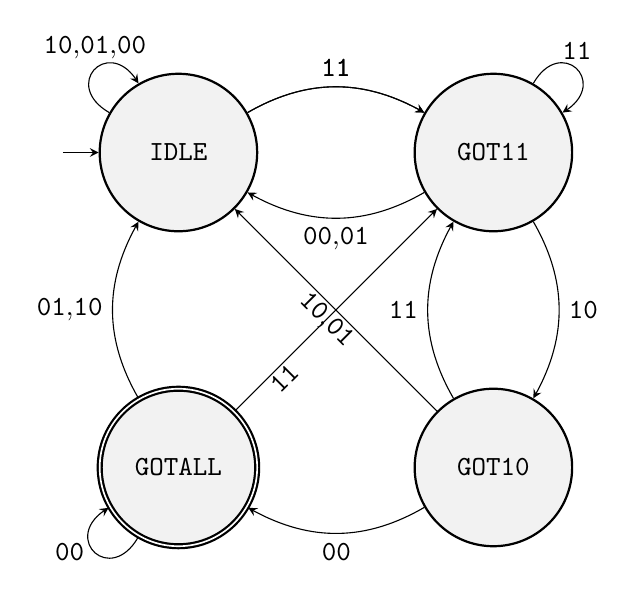
\begin{tikzpicture}
	\tikzset{
	->, % makes the edges directed
	>=stealth, % makes the arrow heads bold
	node distance=4cm, % specifies the minimum distance between two nodes. Change if necessary.
	every state/.style={thick, fill=gray!10}, % sets the properties for each ’state’ node
	initial text=$ $ % sets the text that appears on the start arrow
	}
	\node[state, initial, minimum size=2cm] (idle) {\texttt{IDLE}};
	\node[state, right of=idle, minimum size=2cm] (got11) {\texttt{GOT11}};
	\node[state, below of=got11, minimum size=2cm] (got10) {\texttt{GOT10}};
	\node[state, accepting, below of=idle, minimum size=2cm] (gotall) {\texttt{GOTALL}};
	\draw[->,every loop/.style={looseness=3.5}]
	(idle)  edge[in=120,out=150, loop, above=0.3] node{\texttt{10},\texttt{01},\texttt{00}} (idle)
	(idle)  edge[right, bend left, above=0.3] node{\texttt{11}} (got11)
	(got11) edge[left,  bend left, below=0.3] node{\texttt{00},\texttt{01}} (idle)
	(idle)  edge[right, bend left, above=0.3] node{\texttt{11}} (got11)
	
	(got11)  edge[out=60,in=30, loop, above=0.3] node{\texttt{11}} (got11)
	(got11)  edge[below, bend left, right=0.3]   node{\texttt{10}} (got10)
	(got10)  edge[above, bend left, left=0.3]    node{\texttt{11}} (got11)
	
	(got10)  edge[left, bend left, below=0.3]    node{\texttt{00}} (gotall)
	(gotall)  edge[in=210,out=240, loop, left=0.3] node{\texttt{00}} (gotall)
	(gotall)  edge[above, bend left, left=0.3] node{\texttt{01},\texttt{10}} (idle)
	;
	
	% Sloped edges
	\begin{scope}[every path/.style={->}, every node/.style={sloped, inner sep=1pt}]
       \draw (got10)  edge[anchor=north] node{\texttt{10},\texttt{01}} (idle);
       \draw (gotall)  edge[pos=0.2, anchor=north] node{\texttt{11}} (got11);
    \end{scope}
	;
\end{tikzpicture}
\caption{State diagram of sequence detecting Moore state machine.}
\label{fig:state-dig}
\end{center}
\end{figure}

Figure \ref{fig:state-dig} shows the flow of the state machine given certain states and inputs. The circles represent the four different states that the machine can be in. \texttt{IDLE} represents the state where the detector is waiting for the first pair in the sequence. The arrow to left of this state denotes that this is the starting state. The machine is put into the \texttt{IDLE} state initially by the active-low asynchronous reset signal \texttt{RST}. The arrows on this graph represent how the state would change given a set of input. For example, the bottom arrow labeled \texttt{00} is pointing from the \texttt{GOT10} state to the \texttt{GOTALL} indicating that if the machine is presently in the \texttt{GOT10} state and recieves an input of \texttt{00}, on the next rising clock edge it would be put into the \texttt{GOTALL} state.\\

After a state diagram is created, a transition table is created to quantitatively describe the functionality of the circuit.

\begin{table}[h]
\renewcommand{\arraystretch}{1.2}
\setlength{\tabcolsep}{12pt}
\caption{Truth Table for mathematical operations \(N^2\) and \(5N\)}
\begin{center}
\begin{tabular}{c||c|c|c|cc}
A B & IDLE  & GOT11 & GOT10  & GOTALL & $Q$\\\hhline{=||=|=|=|=}
0 0 & IDLE  & IDLE  & GOTALL & GOTALL & \multirow{4}{*}{$Q^*$}\\\cline{1-5}
0 1 & IDLE  & IDLE  & IDLE   & IDLE   & \\\cline{1-5}
1 1 & GOT11 & GOT11 & GOT11  & GOT11  & \\\cline{1-5}
1 0 & IDLE  & GOT10 & IDLE   & IDLE   &

\end{tabular}
\end{center}
\label{tab:func}
\end{table}

Table \ref{tab:func} shows the next state given current state and input $A$ and $B$. This table can be used to create a Karnaugh Map to define the functionality. Using the 2-bit state definitions previously described, two K-maps are created for the next value of each bit in the state.

\begin{figure}[h!]
	\begin{subfigure}{.5\textwidth}
		\centering
		\begin{Karnaugh}{AB}{$Q_1Q_0$}
				\contingut{0,0,1,1,
						   0,0,0,0,
						   0,1,0,0,
						   0,0,0,0
						   }
		   \implicant{3}{2}{blue}
		   \implicant{9}{9}{red}
		\end{Karnaugh}
		\caption{K-Map ${Q_1}^*$ function}
		\label{fig:q1}
	\end{subfigure}
	\begin{subfigure}{.5\textwidth}
		\centering
		\begin{Karnaugh}{AB}{$Q_1Q_0$}
				\contingut{0,0,0,0,
						   0,0,0,0,
						   0,1,0,0,
						   1,1,1,1
						   }
		   \implicant{12}{14}{yellow}
		   \implicant{13}{9}{green}
		\end{Karnaugh}
		\caption{K-Map ${Q_0}^*$ function}
		\label{fig:q0}
	\end{subfigure}
	
	\caption{K-Maps for next state functions.}
	\label{fig:kmap}
\end{figure}

Using the K-maps shown in Figure \ref{fig:kmap} a set of min-terms can be extracted from the groupings shown. An equation for each next-state bit is required as well as an equation to describe the output \texttt{Z}.

\begin{align}
{Q_1}^* &= \widebar{A}\widebar{B}Q_1 + A\widebar{B}\widebar{Q_1}Q_0\\
&= \widebar{B}(\widebar{A}Q_1 + A\widebar{Q_1}Q_0)\\
{Q_0}^* &= AB + A\widebar{Q_1}Q_0\\
Z &= Q_1\widebar{Q_0}
\end{align}

Equations 1-3 were extracted directly from the K-maps. Equation 3 was not fully simplified so that the output of one of the gates could be reused in both the ${Q_1}^*$ and ${Q_0}^*$ functions. The $Z$ function is a function of only the state as per the definition of a Moore function.\\

Given the next-state functions as boolean expressions of the input and the current state, a circuit schematic can be implemented.

\begin{figure}[h!]
	\centering
	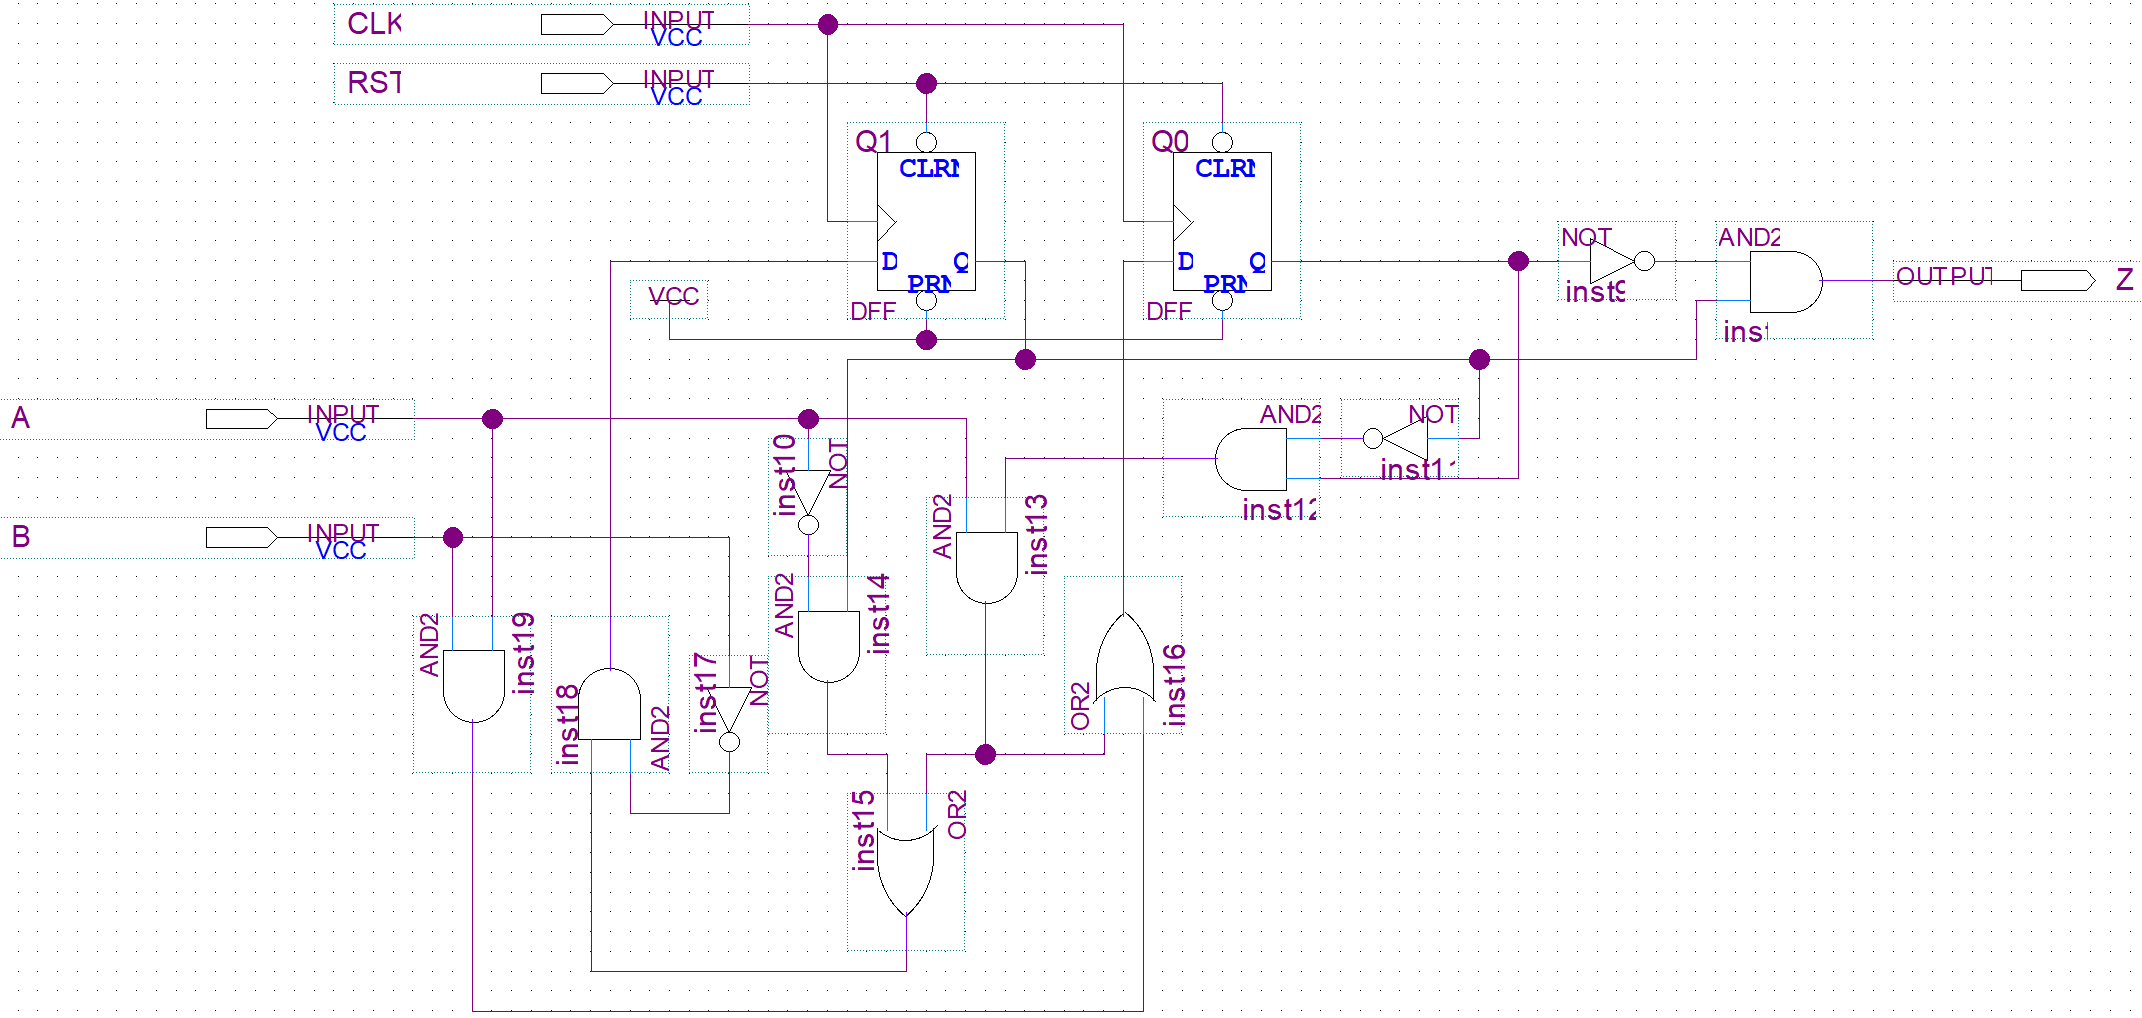
\includegraphics[width=\textwidth]{schematic}
	\caption{State machine circuit schematic.}
	\label{fig:schem-aoi}
\end{figure}

Figure \ref{fig:schem-aoi} shows the circuit implementation of the functions defined in the equations above. An asynchronous reset input pin was added to reset the state before taking an input sequence. The asynchronous set pins on the two D flip-flops are connected to $5\,\si\volt$ source to keep the circuit from using this.

\section*{Results and Analysis}

The circuit implemented in Quartus was tested using Modelsim to verify the integrity of the functions. Two different cases were used to test the functionality. The function test sequence used was given while the second was created to illustrate the full use of the state machine. The following two sequences were used:

\begin{enumerate}
\item (A,B) = (1,1),(1,0),(0,0),(1,0),(0,0),(1,1),(1,0),(0,0),(0,0)
\item (A,B) = (0,1),(0,0),(1,0),(1,1),(1,1),(1,0),(1,1),(1,0),(0,0),(0,0),(1,1)
\end{enumerate}

The second sequence will test every state and transition as well as hold the output to \texttt{HIGH} before moving back to a low state. Both sequences were tested using Modelsim and the wave captures were recorded.
\pagebreak

\begin{figure}[h!]
	\centering
	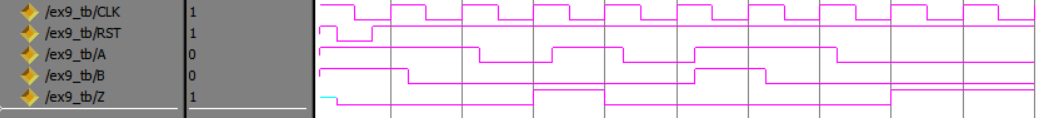
\includegraphics[width=\textwidth]{part1}
	\caption{Wave capture of the first sequence.}
	\label{fig:cap1}
\end{figure}
\begin{figure}[h!]
	\centering
	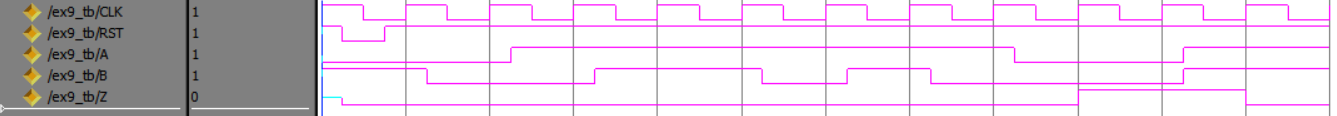
\includegraphics[width=\textwidth]{part2}
	\caption{Wave capture of the second sequence.}
	\label{fig:cap2}
\end{figure}

The wave captures yielded the correct set of outputs. This indicates that the circuit schematic was correct.\\

The timing of this circuit is important when finding the constraints of it. The minimum clock period can be described as the sum of all of the delays measured in the circuit.

\begin{align}
\label{eq:tmin}
T_{min} &= t_{co} + t_{pd} + t_s = 6.232\,ns + 0\,ns + 2.004\,ns = 8.236\,ns \\
\label{eq:fmax}
f_{max} &= \frac{1}{T_{min}} = \frac{1}{8.236 \cdot 10^{-6}} = 121.4\,kHz
\end{align}

The Equation \ref{eq:tmin} indicated the minimum clock period which can be used to calculate the maximum clock frequency of $121.4\,kHz$.

\section*{Conclusion}

In this laboratory exercise, the synthesis of a state machine was reviewed. A state diagram was created which then generated a state table. The state table allowed the creation of a K-map. From the K-map the boolean functions describing the next state could be extracted and a circuit could be implemented in Quartus. The circuit was then tested using two different input sequences in Modelsim. Finally, maximum frequency was calculated using measured delays from quartus. This exercise was successful as the desired functionality described in the lab prompt was achieved by the state machine.

\pagebreak

\section*{Questions}

\begin{enumerate}
\item Repeat the synthesis of the process of your state machine for the following state encoding style.

\begin{table}[h!]
\renewcommand{\arraystretch}{1.2}
\setlength{\tabcolsep}{12pt}
\caption{Alternative states and encodings for the Moore state machine}
\begin{center}
\vspace{-0.5cm}
\begin{tabular}{ccc}
\multirow{2}{*}{State name}& \multicolumn{2}{c}{State}\\
& Q1 & Q0\\\cline{1-3}
Idle  & 0 & 0\\
Got11 & 0 & 1\\
Got10 & 1 & 0\\
GotAll & 1 & 1

\end{tabular}
\end{center}
\label{tab:func}
\end{table}

The state diagram and next-state table can be reused from the previous design. A new set of K-maps and equations however must be created.

\begin{figure}[h!]
	\begin{subfigure}{.5\textwidth}
		\centering
		\begin{Karnaugh}{AB}{$Q_1Q_0$}
				\contingut{0,0,1,1,
						   0,0,0,0,
						   0,1,0,0,
						   0,0,0,0
						   }
		   \implicant{3}{2}{blue}
		   \implicant{9}{9}{red}
		\end{Karnaugh}
		\caption{K-Map ${Q_1}^*$ function}
		\label{fig:q1-2}
	\end{subfigure}
	\begin{subfigure}{.5\textwidth}
		\centering
		\begin{Karnaugh}{AB}{$Q_1Q_0$}
				\contingut{0,0,1,1,
						   0,0,0,0,
						   0,0,0,0,
						   1,1,1,1
						   }
		   \implicant{12}{14}{yellow}
		   \implicant{3}{2}{green}
		\end{Karnaugh}
		\caption{K-Map ${Q_0}^*$ function}
		\label{fig:q0-2}
	\end{subfigure}
	
	\caption{K-Maps for next state functions.}
	\label{fig:kmap-2}
\end{figure}

The first K-map (Figure \ref{fig:q1-2}) is identical to the one in Figure \ref{fig:q1} because the first bit definition is same across all of the states. The second K-map is slightly different to accomodate the change. The equations for the next states can now be extracted.

\begin{align}
{Q_1}^* &= \widebar{A}\widebar{B}Q_1 + A\widebar{B}\widebar{Q_1}Q_0\\
&= \widebar{B}(\widebar{A}Q_1 + A\widebar{Q_1}Q_0)\\
{Q_0}^* &= AB + \widebar{A}\widebar{B}Q_1\\
Z &= Q_1Q_0
\end{align}

${Q_1}^*$ is the same function as before. ${Q_0}^*$ is slightly different from the old function. $Z$ was changed to still only be high when the state is \texttt{GOTALL}.

\begin{figure}[h!]
	\centering
	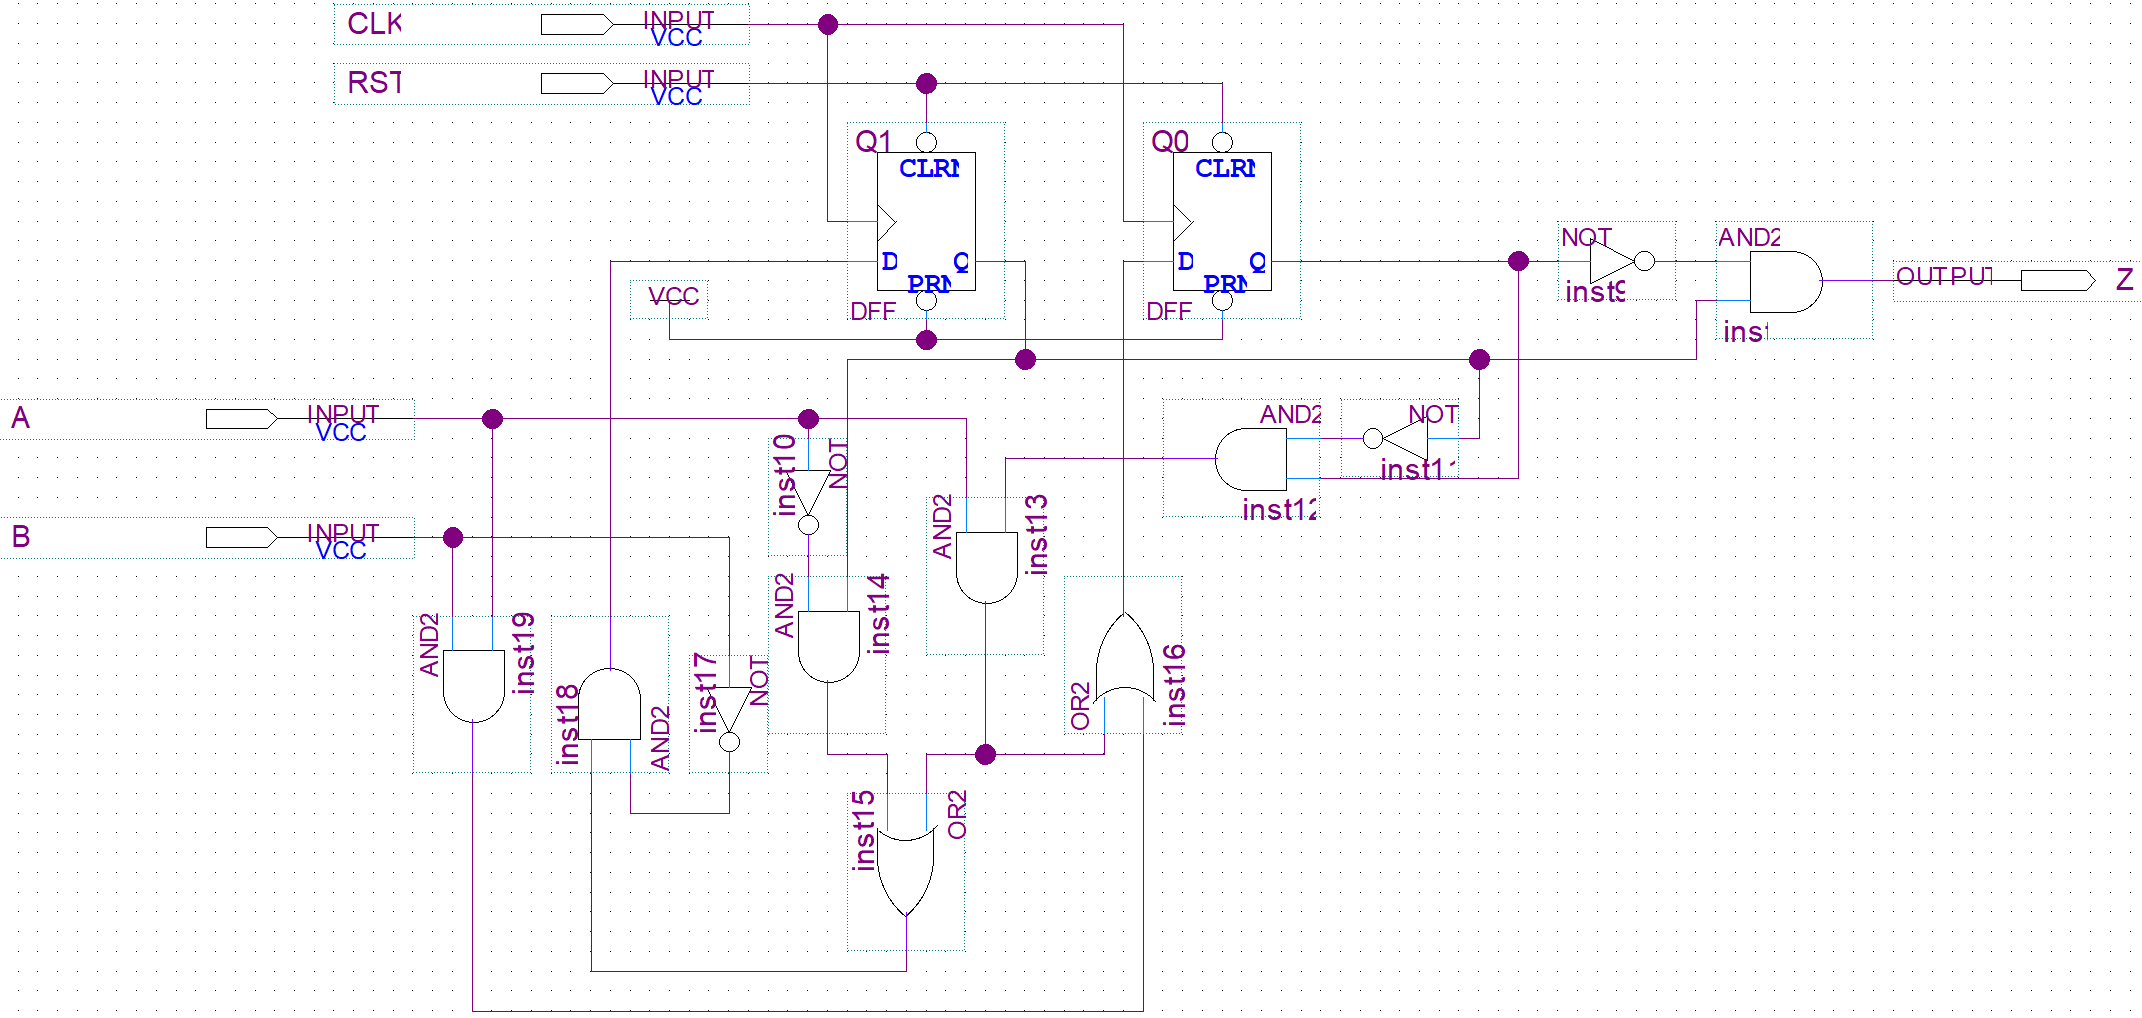
\includegraphics[width=\textwidth]{schematic}
	\caption{State machine circuit schematic with altered encoding.}
	\label{fig:schem-q1}
\end{figure}

\item How many different ways are there to encode a state machine with four states that is implemented using two D flip-flops? Note that the answer should be a number, not ``one-hot'' or ``gray''.

There are $4!$ or $24$ different combinations of encodings that can be used to a encode a state machine with four states.

\item What is ``one-hot'' encoding style?

One hot encoding is useful because it is easier to implement than other types of encoding. In ``one-hot'' encoding, if there are $N$ states, there must be $N$ flip-flops. Each flip-flop will represent a single state. All other flip-flops must be in the low state when one is high. 

\end{enumerate}
\end{document}
